In \eqref{eq:conics/30/def},
substituting
\begin{align}
\vec{q} = \myvec{x\\y}\,
\vec{F} = \myvec{1\\-1}\,
	e = \frac{1}{2},
	\\
	4\sbrak{\brak{x+1}^2 + \brak{y-1}^2}= \brak{\frac{x - y + 3}{\sqrt{1^2 + (-1)^2}}}^2\\
	= \brak{\frac{x - y + 3}{\sqrt{2}}}^2
\end{align}
yielding
\begin{align}
	7\brak{x^2+y^2} + 2xy + 10\brak{-x+y} + 7 = 0 \label{acconiceq}
\end{align}
Comparing the above with
    \eqref{eq:conic_quad_form},
\begin{align}
	\vec{V} = \myvec{{7} & {1} \\  {1} & {7}},
	\,
	\vec{u} ={5}  \myvec{ -1 \\ 1},
	\,
	f = {7}.
\end{align}
The above can also be obtained from 
  \eqref{eq:conic_quad_form_v} -
\eqref{eq:conic_quad_form_f}
using the parameters in 
	\tabref{tab1-1.9-6}.
\begin{table}[H]    
	\centering
	\begin{tabular}[12pt]{ |c| c| c|}
    \hline
    \textbf{Variable} & \textbf{Description} & \textbf{Value}\\
	\hline
	$\vec{n}$ &Normal of Directrix& $\myvec{1 \\ -1} $\\
	\hline
	$\vec{c}$ & c of Directrix& $ 3$\\
	\hline
	$\vec{e}$ & Eccentricity of conic & $\frac{1}{2}$\\
	\hline
	$\vec{F}$ & Focus of conic &  $\myvec{1 \\ -1}$ \\
	\hline
\end{tabular}

	\caption{}
	\label{tab1-1.9-6}
\end{table}
The eigenvalues of $\vec{V}$ are obtained using
	\begin{align}
		\mydet{\vec{V}  - \lambda\vec{I}}  = 0,&\\
		\implies		\mydet{{7} - \lambda& {1}\\ {1} & {7} - \lambda} =0& \\
		\text{or, }\lambda^2 - 14\lambda +48 =0&
		\\
		\implies
		\lambda_1, \lambda_2 = 6, 8&\\
	\end{align}
	The eigenvector of $\vec{V}$ corresponding to $\lambda = 6$ is obtained as
\begin{align}
	\myvec{{7} - \lambda& {1}\\ {1} & {7} - \lambda}\vec{x} =0 &\\
\implies 
	\myvec{1 & 1\\ 1 & 1}\vec{x} =0 &\\
	\implies \vec{x} = \myvec{-1 \\ 1}&
\end{align}
Similarly, the eigenvector corresponding to $\lambda = 8$ can be obtained as
\begin{align}
	\vec{x} = \myvec{1 \\ 1}
\end{align}
resulting in the spectral decomposition
\begin{align}
	\myvec{{7} & {1} \\  {1} & {7}}&=\myvec{ - \frac{1}{\sqrt{2}} & \frac{1}{\sqrt{2}} \\ \frac{1}{\sqrt{2}} & \frac{1}{\sqrt{2}} }
	\myvec{6 & 0 \\ 0 & 8}
\myvec{ - \frac{1}{\sqrt{2}} & \frac{1}{\sqrt{2}} \\ \frac{1}{\sqrt{2}} & \frac{1}{\sqrt{2}} }
\\
	\text{or, }	\vec{V} &= \vec{P}\vec{D}\vec{P^\top}, \quad \vec{P}^\top \vec{P}= \vec{I}
\end{align}
Also, 
\begin{align}
	\vec{P} &= \myvec{\cos\theta & -\sin\theta \\ \sin\theta & \cos\theta}
\\
	\implies \theta &=\frac{3\pi}{4}
\end{align}
%	Using the affine transformation in \eqref{eq:conic_affine},
    From  
      \eqref{eq:f0}
      and
    \eqref{eq:formulae-conic_nonparab_c},
    the corresponding standard ellipse parameters are
\begin{align}
	f_0 &= \vec{u}^\text{T}\vec{V}^{-1}\vec{u} - f  = \frac{25}{48} \myvec{-1 & 1} \myvec{{7} & {-1} \\  {-1} & {7}}  \myvec{-1 \\ 1}  - 7=  \frac{4}{3}\\
	\vec{c} &= -\vec{V}^{-1}\vec{u} = -\frac{5}{48}   \myvec{{7} & {-1} \\  {-1} & {7}}\myvec{ -1 \\ 1} = \frac{5}{6}  \myvec{ 1 \\ -1}
\end{align}
yielding the standard form of the ellipse from 
\eqref{eq:conic_simp_temp_nonparab} as
  \begin{align}
	    \vec{y}^{\top}\brak{\frac{\vec{D}}{f_0}}\vec{y} &= 1   
	    \\
	    \implies
		\vec{y}^\text{T}\myvec{ \frac{9}{2} & 0 \\ 0 & 6}\vec{y} &= 1
\end{align}
From 
\eqref{eq:chord-len-major}
and
\eqref{eq:chord-len-minor},
the lengthes of the axes of are obtained as
\begin{align}
	a &= \sqrt{\frac{f_0}{\lambda_1}} =  \sqrt{\frac{2}{9}}\\
	b &= \sqrt{\frac{f_0}{\lambda_2}} = \sqrt{\frac{1}{6}}
\end{align}
and 
from
			\eqref{eq:latus-ellipse},
the length of the 
latus rectum of the ellipse is
\begin{align}
	l = 2\frac{\sqrt{\abs{f_0 \lambda_1}}}{\lambda_2} = \frac{1}{\sqrt{2}}.
\end{align}
From 
	  \eqref{eq:major-minor-axis-quad},
	  the equations of the axes are
\begin{align}
	\text{Minor Axis}:&   \myvec{- \frac{1}{\sqrt{2}} & \frac{1}{\sqrt{2}}}x\vec{x} &= 0\\
	\text{Major Axis}:&   \myvec{\frac{1}{\sqrt{2}} & \frac{1}{\sqrt{2}}}\vec{x} &= 0
\end{align}
See \figref{fig:fig1} for verification.
%
\begin{figure}[H]
	\centering
	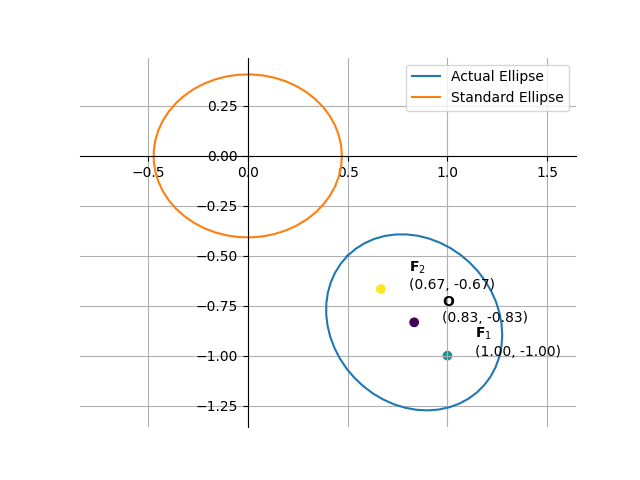
\includegraphics[width=0.75\columnwidth]{chapters/11/11/5/Figures/fig1.png} 
	\caption{}
	\label{fig:fig1}
\end{figure} 

